\def\bmode{0} % Mode 0 for presentation, mode 1 for a handout with notes, mode 2 for handout without notes
\if 0\bmode
\documentclass[smaller]{beamer}
\else \if 1\bmode
\immediate\write18{pdflatex -jobname=\jobname-Notes-Handout\space\jobname}
\documentclass[smaller,handout]{beamer}
\usepackage{handoutWithNotes}
\pgfpagesuselayout{2 on 1 with notes}[letterpaper, landscape, border shrink=4mm]
\else \if 2\bmode
\immediate\write18{pdflatex -jobname=\jobname_Handout\space\jobname}
\documentclass[smaller,handout]{beamer}
\fi
\fi
\fi
%\documentclass[smaller, handout]{beamer}


% \documentclass[smaller,handout
% ]{beamer}
%\usepackage{etex}
%\newcommand{km}{6{} }

% \usetheme[
%   outer/progressbar=foot,
%   outer/numbering=counter,
%  block=fillFF
% ]{metropolis}

%\useoutertheme{metropolis}

\usetheme{Madrid}
\useoutertheme[subsection=false]{miniframes} % Alternatively: miniframes, infolines, split
\useinnertheme{circles}
\usecolortheme{seahorse}

\usepackage[backend=biber,style=authoryear,maxcitenames=2,maxbibnames=99,safeinputenc,url=false,
eprint=false]{biblatex}
\addbibresource{bib/references.bib}
\AtEveryCitekey{\iffootnote{{\tiny}\tiny}{\tiny}}
\usepackage{appendixnumberbeamer}
%\usepackage{pgfpages}
%\setbeameroption{hide notes} % Only slides
%\setbeameroption{show only notes} % Only notes
%\setbeameroption{hide notes} % Only notes
%\setbeameroption{show notes on second screen=right} % Both

% \usepackage[sfdefault]{Fira Sans}

% \setsansfont[BoldFont={Fira Sans}]{Fira Sans Light}
% \setmonofont{Fira Mono}

%\usepackage{fira}
%\setsansfont{Fira}
%\setmonofont{Fira Mono}
% To give a presentation with the Skim reader (http://skim-app.sourceforge.net) on OSX so
% that you see the notes on your laptop and the slides on the projector, do the following:
% 
% 1. Generate just the presentation (hide notes) and save to slides.pdf
% 2. Generate onlt the notes (show only nodes) and save to notes.pdf
% 3. With Skim open both slides.pdf and notes.pdf
% 4. Click on slides.pdf to bring it to front.
% 5. In Skim, under "View -> Presentation Option -> Synhcronized Noted Document"
%    select notes.pdf.
% 6. Now as you move around in slides.pdf the notes.pdf file will follow you.
% 7. Arrange windows so that notes.pdf is in full screen mode on your laptop
%    and slides.pdf is in presentation mode on the projector.

% Give a slight yellow tint to the notes page
%\setbeamertemplate{note page}{\pagecolor{yellow!5}\insertnote}\usepackage{palatino}


%\usetheme{metropolis}
%\usecolortheme{beaver}
\usepackage{xcolor}
\definecolor{darkcandyapplered}{HTML}{A40000}
\definecolor{lightcandyapplered}{HTML}{e74c3c}

%\setbeamercolor{title}{fg=darkcandyapplered}
%\setbeamercolor{frametitle}{bg=darkcandyapplered!80!black!90!white}
%\setbeamertemplate{frametitle}{\bf\insertframetitle}
%\setbeamercolor{footnote mark}{fg=darkcandyapplered}
%\setbeamercolor{footnote}{fg=darkcandyapplered!70}
%\Raggedbottom
%\setbeamerfont{page number in head/foot}{size=\tiny}
%\usepackage[tracking]{microtype}


\setbeamertemplate{frametitle}{%
    \nointerlineskip%
    \begin{beamercolorbox}[wd=\paperwidth,ht=2.0ex,dp=0.6ex]{frametitle}
        \hspace*{1ex}\insertframetitle%
    \end{beamercolorbox}%
}



\setbeamerfont{caption}{size=\footnotesize}
\setbeamercolor{caption name}{fg=darkcandyapplered}


%\usepackage[sc,osf]{mathpazo}   % With old-style figures and real smallcaps.
%\linespread{1.025}              % Palatino leads a little more leading

% Euler for math and numbers
%\usepackage[euler-digits,small]{eulervm}
%\AtBeginDocument{\renewcommand{\hbar}{\hslash}}
\usepackage{graphicx,multirow,paralist,booktabs}


%\mode<presentation> { \setbeamercovered{transparent} }

\setbeamertemplate{navigation symbols}{}
\makeatletter
\def\beamerorig@set@color{%
  \pdfliteral{\current@color}%
  \aftergroup\reset@color
}
\def\beamerorig@reset@color{\pdfliteral{\current@color}}
\makeatother

%=== GRAPHICS PATH ===========
\graphicspath{{./m5-images/}}
% Marginpar width
%Marginpar width
%\setlength{\marginparsep}{.02in}


%% Captions
% \usepackage{caption}
% \captionsetup{
%   labelsep=quad,
%   justification=raggedright,
%   labelfont=sc
% }

%AMS-TeX packages

\usepackage{amssymb,amsmath,amsthm} 
\usepackage{bm}
\usepackage{color}

\usepackage{hyperref,enumerate}
\usepackage{minitoc,array}


%https://tex.stackexchange.com/a/31370/2269
\usepackage{mathtools,cancel}

\renewcommand{\CancelColor}{\color{red}} %change cancel color to red

\makeatletter
\let\my@cancelto\cancelto %copy over the original cancelto command
\newcommand<>{\cancelto}[2]{\alt#3{\my@cancelto{#1}{#2}}{\mathrlap{#2}\phantom{\my@cancelto{#1}{#2}}}}
% redefine the cancelto command, using \phantom to assure that the
% result doesn't wiggle up and down with and without the arrow
\makeatother


\definecolor{slblue}{rgb}{0,.3,.62}
\hypersetup{
    colorlinks,%
    citecolor=blue,%
    filecolor=blue,%
    linkcolor=blue,
    urlcolor=slblue
}

%%% TIKZ
\usepackage{animate}
\usepackage{tikz}
\usepackage{pgfplots}
\usepackage{pgfplotstable}
\usepackage{pgfgantt}
\usepackage{tikzsymbols}
\pgfplotsset{compat=newest}
\usepgfplotslibrary{groupplots,fillbetween}

\usetikzlibrary{arrows,shapes,positioning,shapes.geometric}
\usetikzlibrary{decorations.markings}
\usetikzlibrary{shadows,automata}
\usetikzlibrary{patterns,matrix}
\usetikzlibrary{trees,mindmap,backgrounds}
%\usetikzlibrary{circuits.ee.IEC}
\usetikzlibrary{decorations.text}
% For Sagnac Picture
\usetikzlibrary{%
    decorations.pathreplacing,%
    decorations.pathmorphing%
}
\tikzset{no shadows/.style={general shadow/.style=}}
%
%\usepackage{paralist}



%%% FORMAT PYTHON CODE
%\usepackage{listings}
% Default fixed font does not support bold face
\DeclareFixedFont{\ttb}{T1}{txtt}{bx}{n}{8} % for bold
\DeclareFixedFont{\ttm}{T1}{txtt}{m}{n}{8}  % for normal

% Custom colors
\definecolor{deepblue}{rgb}{0,0,0.5}
\definecolor{deepred}{rgb}{0.6,0,0}
\definecolor{deepgreen}{rgb}{0,0.5,0}
 

\usepackage{listings}

% % Python style for highlighting
\newcommand\pythonstyle{\lstset{
language=Python,
basicstyle=\normalsize\ttm\color{blue},       % Changed from \footnotesize to \normalsize
otherkeywords={self},             % Add keywords here
keywordstyle=\normalsize\ttb\color{purple},  % Changed from \footnotesize
emph={MyClass,__init__},          % Custom highlighting
emphstyle=\normalsize\ttb\color{deepred},      % Changed from \footnotesize
stringstyle=\color{deepgreen},
commentstyle=\color{deepgreen},   % Make comments green
frame=tb,                         % Any extra options here
backgroundcolor=\color{gray!20},  % Added gray background
showstringspaces=false            % 
}}

% Python environment
\lstnewenvironment{python}[1][]
{
\pythonstyle
\lstset{#1}
}
{}

% % Python for external files
\newcommand\pythonexternal[2][]{{
\pythonstyle
\lstinputlisting[#1]{#2}}}

% % Python for inline
\newcommand\pythoninline[1]{{\pythonstyle\lstinline!#1!}}


\newcommand{\osn}{\oldstylenums}
\newcommand{\dg}{^{\circ}}
\newcommand{\lt}{\left}
\newcommand{\rt}{\right}
\newcommand{\pt}{\phantom}
\newcommand{\tf}{\therefore}
\newcommand{\?}{\stackrel{?}{=}}
\newcommand{\fr}{\frac}
\newcommand{\dfr}{\dfrac}
\newcommand{\ul}{\underline}
\newcommand{\tn}{\tabularnewline}
\newcommand{\nl}{\newline}
\newcommand\relph[1]{\mathrel{\phantom{#1}}}
\newcommand{\cm}{\checkmark}
\newcommand{\ol}{\overline}
\newcommand{\rd}{\color{red}}
\newcommand{\bl}{\color{blue}}
\newcommand{\pl}{\color{purple}}
\newcommand{\og}{\color{orange!90!black}}
\newcommand{\gr}{\color{green!40!black}}
\newcommand{\nin}{\noindent}
\newcommand{\la}{\lambda}
\renewcommand{\th}{\theta}
\newcommand{\al}{\alpha}
\newcommand{\G}{\Gamma}
\newcommand*\circled[1]{\tikz[baseline=(char.base)]{
            \node[shape=circle,draw,thick,inner sep=1pt] (char) {\small #1};}}

\newcommand{\bc}{\begin{compactenum}[\quad--]}
\newcommand{\ec}{\end{compactenum}}

\newcommand{\p}{\partial}
\newcommand{\pd}[2]{\frac{\partial{#1}}{\partial{#2}}}
\newcommand{\dpd}[2]{\dfrac{\partial{#1}}{\partial{#2}}}
\newcommand{\pdd}[2]{\frac{\partial^2{#1}}{\partial{#2}^2}}
\newcommand{\nmfr}[3]{\Phi\left(\frac{{#1} - {#2}}{#3}\right)}


\pgfmathdeclarefunction{poiss}{1}{%
  \pgfmathparse{(#1^x)*exp(-#1)/(x!)}%
  }

\pgfmathdeclarefunction{gauss}{2}{%
  \pgfmathparse{1/(#2*sqrt(2*pi))*exp(-((x-#1)^2)/(2*#2^2))}%
}

\pgfmathdeclarefunction{expo}{2}{%
  \pgfmathparse{#1*exp(-#1*#2)}%
}

\pgfmathdeclarefunction{expocdf}{2}{%
  \pgfmathparse{1 -exp(-#1*#2)}%
}

% \makeatletter
% \long\def\ifnodedefined#1#2#3{%
%     \@ifundefined{pgf@sh@ns@#1}{#3}{#2}%
% }

% \pgfplotsset{
%     discontinuous/.style={
%     scatter,
%     scatter/@pre marker code/.code={
%         \ifnodedefined{marker}{
%             \pgfpointdiff{\pgfpointanchor{marker}{center}}%
%              {\pgfpoint{0}{0}}%
%              \ifdim\pgf@y>0pt
%                 \tikzset{options/.style={mark=*, fill=white}}
%                 \draw [densely dashed] (marker-|0,0) -- (0,0);
%                 \draw plot [mark=*] coordinates {(marker-|0,0)};
%              \else
%                 \tikzset{options/.style={mark=none}}
%              \fi
%         }{
%             \tikzset{options/.style={mark=none}}        
%         }
%         \coordinate (marker) at (0,0);
%         \begin{scope}[options]
%     },
%     scatter/@post marker code/.code={\end{scope}}
%     }
% }

% \makeatother

\renewcommand{\arraystretch}{1.5}
%%%%%%%%%%%%%%%%%%%%%%%%%%%%%%%%%%%%%%%%%%%%%%%%%%%
%%%%%%%%%%%%%%%%%%%%%%%%%%%%%%%%%%%%%%%%%%%%%%%%%%%

\title[CEE 260/MIE 273 M5c: Goodness of Fit]{{\normalsize CEE 260/MIE 273: Probability and Statistics in Civil Engineering} \\
Lecture M5c: Goodness of Fit Testing; Chi-square}
\date[\today]{\footnotesize \today}
\author{{\bf Jimi Oke}}
\institute[UMass Amherst]{
  \begin{tikzpicture}[baseline=(current bounding box.center)]
    \node[anchor=base] at (-7,0) (its) {\includegraphics[scale=.3]{UMassEngineering_vert}} ;
  \end{tikzpicture}
}

\newcommand{\hpp}{\hat{p_1} - \hat{p_2}}
\newcommand{\pp}{p_1 - p_2}    
\begin{document}

\maketitle




\begin{frame}
  \frametitle{Outline}
  \tableofcontents
\end{frame}

 





\begin{frame}
	\frametitle{Today's objectives}
  
	\begin{itemize}
	\item Get introduced to the $\chi^2$ distribution \pause
	\item Conduct $\chi^2$ tests  \pause
	\item Conduct goodness-of-fit tests using the $\chi^2$ distribution
	\end{itemize}
	\pause
	Reading: Section 6.3, Open Intro Statistics
  \end{frame}
  
\section{Introduction}
\begin{frame}
  \frametitle{}

  {\bf Scenario 1:} \\ \pause

  Recall the assumptions made for samples on which we conduct inference:\pause

  \begin{enumerate}
  \item Independence
  \item Normality (i.e.\ if the Central Limit Theorem applies)
  \end{enumerate}
  \pause
  How do we test for these?
  \bigskip

  {\bf Scenario 2:} \\ \pause
  You want to create a focus group for a study which is representative of demographic groups of interest (e.g.\ income, race/ethnicity, education level, major, etc.) How would you evaluate whether your sample is representative/balanced or biased toward a certain group? \pause

  \begin{tabular}{c c c c c c}\toprule
    Group & A & B & C & D & Total \\\midrule
    Observed counts & $\hat{n}_A$ & $\hat{n}_B$ & $\hat{n}_C$ & $\hat{n}_D$ &  \\\midrule
    Expected counts & $n_A$ & $n_B$ & $n_C$ & $n_D$ & \\\bottomrule
  \end{tabular}
\end{frame}

\begin{frame}
  \frametitle{Scenario 2 (cont.)}\pause

  If we define a test statistic $\chi^2$ as:
  \begin{equation}
    \chi^2 = Z_A^2 + Z_B^2 + Z_C^2 + Z_D^2
  \end{equation}
\pause
where:
\pause
\begin{equation}
  Z_A^2 = \fr{(\hat{n}_A - n_A )^2}{n_A} = \fr{(\text{observed count} - \text{expected count})^2}{\text{expected count}}
\end{equation}
\pause
and so on, then it turns out that $\chi^2$ follows a special distribution called the $\chi^2$ distribution
\end{frame}
\begin{frame}
  \frametitle{Chi-square testing}
  The \textbf{chi-square} ($\chi^2$) test provides a framework to judge: \pause
  \begin{enumerate}
	\item if categories of two factors occur \textbf{independently} of each other in a population  \pause
	\item proportions in different categories are the same for all populations (homogeneity) \pause
  \item fitness of the frequency of observations from a multinomial experiment (i.e. multiple outcomes) to  specified probabilities \pause
  \item more generally, the fitness of a theoretical probability distribution model to  an experimental dataset
  \end{enumerate}
  \pause
  To conduct chi-square tests, we use the $\chi^2$ distribution, \pause whose properties we can exploit for statistical inference (hypothesis testing, and so on)
\end{frame}



\section{Chi-square distribution}

\begin{frame}
  \frametitle{The chi-square distribution} \pause
  The chi-square ($\chi^2$) distribution is specifed as $\chi^2(k)$  or $\chi^2_k$, where $k$ is the single parameter called \textbf{degrees of freedom} (or ``df'').
  \pause
        \begin{tikzpicture}[scale=1,
      declare function={
        gamma(\z)=2.506628274631*sqrt(1/\z)+ 0.20888568*(1/\z)^(1.5)+ 0.00870357*(1/\z)^(2.5)- (174.2106599*(1/\z)^(3.5))/25920- (715.6423511*(1/\z)^(4.5))/1244160)*exp((-ln(1/\z)-1)*\z;
      },
      declare function={
        beta(\x,\y)=gamma(\x)*gamma(\y)/gamma(\x+\y);
      },
      declare function={
        fdst(\x,\a,\b) = 1 / beta(\a/2, \b/2) * (\a/\b)^(\a/2) * \x^(\a/2-1) * (1 + \a/\b*\x)^(-(\a + \b)/2);
      },
      declare function={
       chisq(\x,\k) = exp((0.5*\k-1.0)*ln(\x) - 0.5*\x - gamma(0.5*\k) - \k*0.5*ln(2));
      }
      ]

      \begin{axis}[
        axis x line=center,
        axis y line=center,
        xlabel=$\chi^2$,
        ylabel={PDF$(\chi^2)$},
        x label style={anchor=west},
        y label style={anchor=south},
        axis lines=left,
        axis on top,
        enlargelimits=upper,
        samples=100,
        xmin=0, ymin=0,
        domain=0.01:15,
        legend cell align=left,
        yticklabel style={
          /pgf/number format/fixed,
          /pgf/number format/fixed zerofill,
          /pgf/number format/precision=2
        },        
        ]

        \only<1->{\addplot [very thick,blue] {chisq(x,2)}; \addlegendentry{$k=1$}}
        \only<2->{\addplot [very thick,orange] {chisq(x,4)}; \addlegendentry{$k=3$}}
        \only<3->{\addplot [very thick,purple] {chisq(x,7)}; \addlegendentry{$k=6$}}
      \end{axis}
    \end{tikzpicture}    
\end{frame}

\begin{frame}
  \frametitle{Chi-square distribution (cont.)}

  \begin{exampleblock}{Example 1: CDF of chi-square distribution}\pause
    Estimate the area under the $\chi^2$ curve where $k = 9$.\pause

          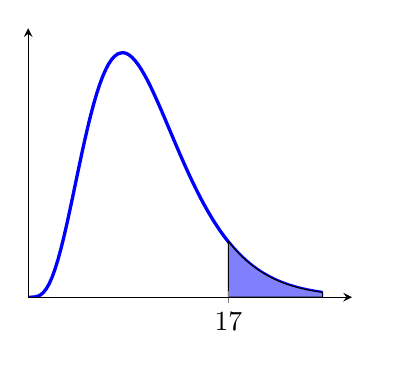
\begin{tikzpicture}[scale=1,
      declare function={
        gamma(\z)=2.506628274631*sqrt(1/\z)+ 0.20888568*(1/\z)^(1.5)+ 0.00870357*(1/\z)^(2.5)- (174.2106599*(1/\z)^(3.5))/25920- (715.6423511*(1/\z)^(4.5))/1244160)*exp((-ln(1/\z)-1)*\z;
      },
      declare function={
       chisq(\x,\k) = exp((0.5*\k-1.0)*ln(\x) - 0.5*\x - gamma(0.5*\k) - \k*0.5*ln(2));
      }
      ]

      \begin{axis}[scale = .6,
        axis x line=center,
        xlabel=$$,
        ytick=\empty,                
        xtick={17},
        xticklabels={17},
        x label style={anchor=west},
        y label style={anchor=south},
        axis lines=left,
        axis on top,
        enlargelimits=upper,
        samples=100,
        xmin=0, ymin=0,
        domain=0.01:25,
        legend cell align=left,
                yticklabel style={
          /pgf/number format/fixed,
          /pgf/number format/fixed zerofill,
          /pgf/number format/precision=2
        },        
        ]
        \addplot [very thick,blue] {chisq(x,10)}; %\addlegendentry{$k=1$}
        \addplot [ fill=blue!50!white,domain=17:25] {chisq(x,10)} \closedcycle ;
        %\draw[<-, thick] (axis cs: 6,.01) -- (axis cs: 8,.02) node [above right] {\og $p$-value $= 0.085$};
        % \addplot [very thick,purple] {chisq(x,7)}; \addlegendentry{$k=6$}
      \end{axis}
    \end{tikzpicture}

    \pause

    \begin{enumerate}[(a)]
    \item 0.05
    \item 0.02
    \item between 0.02 and 0.05
    \item between 0.05 and 0.1
    \item between 0.01 and 0.02
    \end{enumerate}
  \end{exampleblock}
\end{frame}

\begin{frame}
  \frametitle{Chi-square distribution (cont.)}
 \begin{exampleblock}{Example 1: CDF of chi-square distribution (cont.)}\pause
    Estimate the area under the $\chi^2$ curve where $k = 9$.\pause

    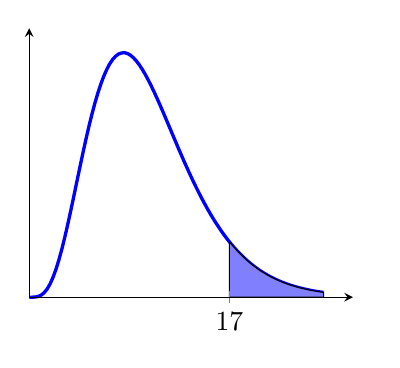
\begin{tikzpicture}[scale=1,
		declare function={
		  gamma(\z)=2.506628274631*sqrt(1/\z)+ 0.20888568*(1/\z)^(1.5)+ 0.00870357*(1/\z)^(2.5)- (174.2106599*(1/\z)^(3.5))/25920- (715.6423511*(1/\z)^(4.5))/1244160)*exp((-ln(1/\z)-1)*\z;
		},
		declare function={
		 chisq(\x,\k) = exp((0.5*\k-1.0)*ln(\x) - 0.5*\x - gamma(0.5*\k) - \k*0.5*ln(2));
		}
		]
  
		\begin{axis}[scale = .6,
		  axis x line=center,
		  xlabel=$$,
		  ytick=\empty,                
		  xtick={17},
		  xticklabels={17},
		  x label style={anchor=west},
		  y label style={anchor=south},
		  axis lines=left,
		  axis on top,
		  enlargelimits=upper,
		  samples=100,
		  xmin=0, ymin=0,
		  domain=0.01:25,
		  legend cell align=left,
				  yticklabel style={
			/pgf/number format/fixed,
			/pgf/number format/fixed zerofill,
			/pgf/number format/precision=2
		  },        clip=false
		  ]
		  \addplot [very thick,blue] {chisq(x,10)}; %\addlegendentry{$k=1$}
		  \addplot [ fill=blue!50!white,domain=17:25] {chisq(x,10)} \closedcycle ;
		  %\draw[<-, thick] (axis cs: 18,.001) -- (axis cs: 19,.01) node [above right] {Area $= 0.0487$};
        % \addplot [very thick,purple] {chisq(x,7)}; \addlegendentry{$k=6$}
      \end{axis}
    \end{tikzpicture}
	\pause

	In Python, you can find the area using \pythoninline{1 - chi2.cdf(17, 9)} $= 0.0487$. \pause

    \pause Answer: (c) between 0.02 and 0.05
  \end{exampleblock}
\end{frame}


\section{Chi-square tests}

\begin{frame}
	\frametitle{Hypothesis testing}
	\pause
	When conducting hypothesis tests using the chi-square distribution, the test is always upper-tailed. \pause

	\begin{itemize}
		\item Test statistic: $\chi^2$ \pause
		\item Null hypothesis: $\chi^2$ follows a chi-square distribution \pause
		\item Alternative hypothesis: $\chi^2$ does not follow a chi-square distribution
	\end{itemize}
	\pause
	\begin{minipage}{.5\textwidth}
		
	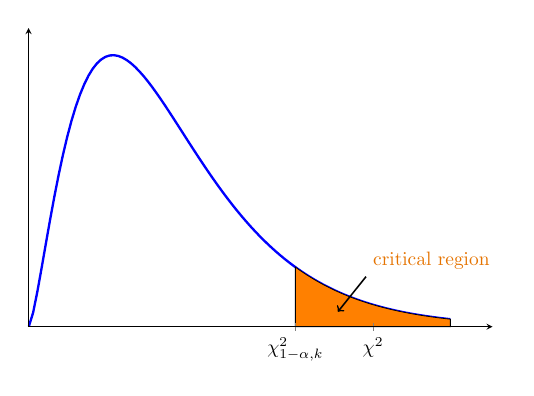
\begin{tikzpicture}[scale=.7,
		declare function={
		  gamma(\z)=2.506628274631*sqrt(1/\z)+ 0.20888568*(1/\z)^(1.5)+ 0.00870357*(1/\z)^(2.5)- (174.2106599*(1/\z)^(3.5))/25920- (715.6423511*(1/\z)^(4.5))/1244160)*exp((-ln(1/\z)-1)*\z;
		},
		declare function={
		 chisq(\x,\k) = exp((0.5*\k-1.0)*ln(\x) - 0.5*\x - gamma(0.5*\k) - \k*0.5*ln(2));
		}
		]
		\begin{axis}[
		  height=7cm, width=10cm,
		  axis x line=center,
		  axis y line=center,
		  xlabel=$$,
		  xtick={9.4877, 12.25},
		  xticklabels={$\chi^2_{1-\alpha,k}$, $\chi^2$},
		  ytick=\empty,
		  x label style={anchor=west},
		  y label style={anchor=south},
		  axis lines=left,
		  axis on top,
		  enlargelimits=upper,
		  samples=100,
		  xmin=0, ymin=0,
		  domain=0.01:15,
		  legend cell align=left,
		  clip=false
		  ]
		  \addplot [very thick,blue] {chisq(x,5)}; %\addlegendentry{$k=1$}
		  \addplot [ fill=orange,domain=9.4877:15] {chisq(x,5)} \closedcycle ;
		  \draw[<-, thick] (axis cs: 11,.003) -- (axis cs: 12,.01) node [above right] {\og critical region};
		  % \addplot [very thick,purple] {chisq(x,7)}; \addlegendentry{$k=6$}
		\end{axis}
	  \end{tikzpicture}    	
	\end{minipage}
	\begin{minipage}{.45\textwidth}
		The critical value is $\chi^2_{1-\alpha,k}$ (\texttt{chi2inv(1 - alpha, nu)}). \pause
		\begin{itemize}
			\item If $\chi^2 > \chi^2_{1-\alpha,k}$, {\bf reject null hypothesis} \pause
			\item If $\chi^2 \leq \chi^2_{1-\alpha,k}$, {\bf fail to reject null hypothesis}
		\end{itemize}
	\end{minipage}

\end{frame}
\begin{frame}
  \frametitle{$p$-values for chi-square tests}\pause

  As our focus is on upper-tailed tests, the $p$-value is given as the area to the right of the test statistic under the chi-square curve (\pythoninline{chi2.sf(test, df)})

      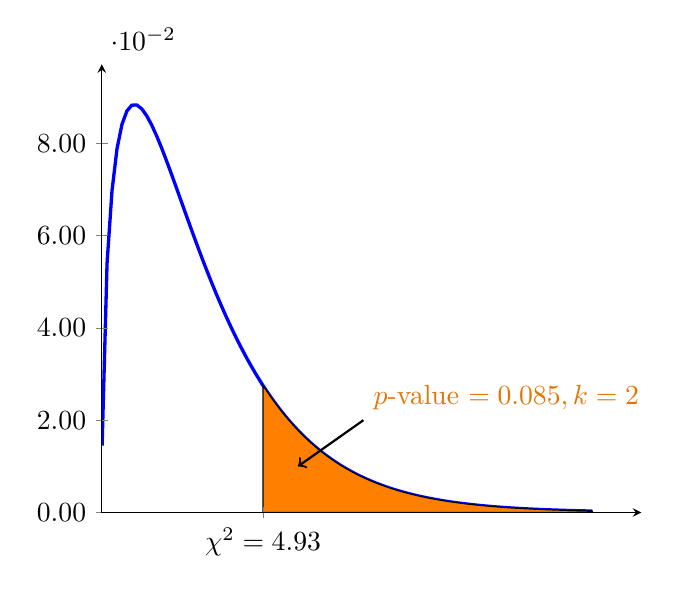
\begin{tikzpicture}[scale=1,
      declare function={
        gamma(\z)=2.506628274631*sqrt(1/\z)+ 0.20888568*(1/\z)^(1.5)+ 0.00870357*(1/\z)^(2.5)- (174.2106599*(1/\z)^(3.5))/25920- (715.6423511*(1/\z)^(4.5))/1244160)*exp((-ln(1/\z)-1)*\z;
      },
      declare function={
       chisq(\x,\k) = exp((0.5*\k-1.0)*ln(\x) - 0.5*\x - gamma(0.5*\k) - \k*0.5*ln(2));
      }
      ]

      \begin{axis}[
        axis x line=center,
        xlabel=$$,
        xtick={4.93},
        %ytick={},
        xticklabel={$\chi^2 = 4.93$},
        x label style={anchor=west},
        y label style={anchor=south},
        axis lines=left,
        axis on top,
        enlargelimits=upper,
        samples=100,
        xmin=0, ymin=0,
        domain=0.01:15,
        legend cell align=left,
                yticklabel style={
          /pgf/number format/fixed,
          /pgf/number format/fixed zerofill,
          /pgf/number format/precision=2
        },        
        ]
        \addplot [very thick,blue] {chisq(x,3)}; %\addlegendentry{$k=1$}
        \addplot [ fill=orange,domain=4.93:15] {chisq(x,3)} \closedcycle ;
        \draw[<-, thick] (axis cs: 6,.01) -- (axis cs: 8,.02) node [above right] {\og $p$-value $= 0.085, k = 2$};
        % \addplot [very thick,purple] {chisq(x,7)}; \addlegendentry{$k=6$}
      \end{axis}
    \end{tikzpicture}    
\end{frame}



\begin{frame}
  \frametitle{Working with the chi-square distribution}
  \begin{exampleblock}{Example 2: Hypothesis testing}\pause
    What conclusion would be appropriate for an upper-tailed chi-square test given the following:\pause
    \begin{eqnarray*}
      \alpha &=& 0.05 \\
      \chi^2 &=& 12.25 \quad \text{\rd (Test statistic)} \\
      k &=& 4 \quad \text{(\bl $\chi^2$ parameter: degrees of freedom)}\\
    \end{eqnarray*}

  \end{exampleblock}
\end{frame}


\begin{frame}
  \frametitle{Working with the chi-square distribution}
  \begin{exampleblock}{Example 2: Hypothesis testing (cont.)}\pause
    The critical value is given by:
    \begin{equation*}
      \chi^2_{1-\alpha,k} = \chi^2_{0.95,4} = \pythoninline{chi2.ppf(.95, 4)} = \pause  9.4877
    \end{equation*}
    \pause
   

	\begin{minipage}{.4\textwidth}
		We compare the test statistic:\pause
		\begin{equation*}
			\chi^2 = 12.25 \pause > \chi^2_{0.95,4} = 9.4877
		  \end{equation*}
	\end{minipage}\pause\quad
	\begin{minipage}{.5\textwidth}
		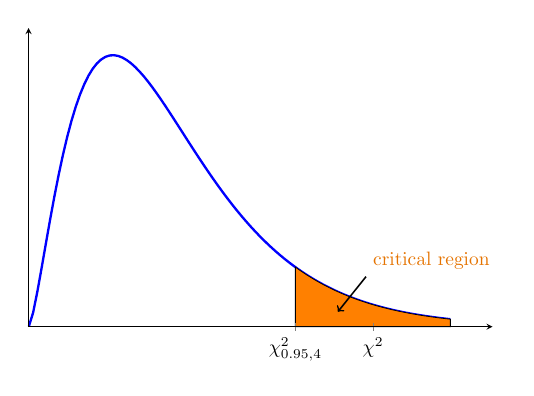
\begin{tikzpicture}[scale=.7,
			declare function={
			  gamma(\z)=2.506628274631*sqrt(1/\z)+ 0.20888568*(1/\z)^(1.5)+ 0.00870357*(1/\z)^(2.5)- (174.2106599*(1/\z)^(3.5))/25920- (715.6423511*(1/\z)^(4.5))/1244160)*exp((-ln(1/\z)-1)*\z;
			},
			declare function={
			 chisq(\x,\k) = exp((0.5*\k-1.0)*ln(\x) - 0.5*\x - gamma(0.5*\k) - \k*0.5*ln(2));
			}
			]
			\begin{axis}[
			  height=7cm, width=10cm,
			  axis x line=center,
			  axis y line=center,
			  xlabel=$$,
			  xtick={9.4877, 12.25},
			  xticklabels={$\chi^2_{0.95,4}$, $\chi^2$},
			  ytick=\empty,
			  x label style={anchor=west},
			  y label style={anchor=south},
			  axis lines=left,
			  axis on top,
			  enlargelimits=upper,
			  samples=100,
			  xmin=0, ymin=0,
			  domain=0.01:15,
			  legend cell align=left,
			  clip=false
			  ]
			  \addplot [very thick,blue] {chisq(x,5)}; %\addlegendentry{$k=1$}
			  \addplot [ fill=orange,domain=9.4877:15] {chisq(x,5)} \closedcycle ;
			  \draw[<-, thick] (axis cs: 11,.003) -- (axis cs: 12,.01) node [above right] {\og critical region};
			  % \addplot [very thick,purple] {chisq(x,7)}; \addlegendentry{$k=6$}
			\end{axis}
		  \end{tikzpicture}    		  
	\end{minipage}
    \pause

    The test statistic is in the critical region. \pause We therefore \textbf{reject the null hypothesis}.
  \end{exampleblock}
\end{frame}

 


\begin{frame}
  \frametitle{Working with the chi-square distribution (cont.)}
  \begin{exampleblock}{Example 3: $p$-value}\pause
    Give as much information as you can about the $p$-value for an upper-tailed chi-square test in this situation:\pause
    \begin{eqnarray*}
      k &=& 4 \\
      \chi^2 &=& 7.5
    \end{eqnarray*}
  \end{exampleblock}
\end{frame}

\begin{frame}
  \frametitle{Working with the chi-square distribution (cont.)}
  \begin{exampleblock}{Example 3: $p$-value (cont.)}\pause

    First, we can look up the critical value at a given significance level.\pause

    Let us choose $\alpha = 0.05$. \pause The critical value is given by:\pause
    \begin{equation*}
      \chi^2_{0.95,4} =  {\og \mathtt{chi2inv(.95, 4)}} = 9.4877
    \end{equation*}

    \pause

	\begin{minipage}{.5\textwidth}
	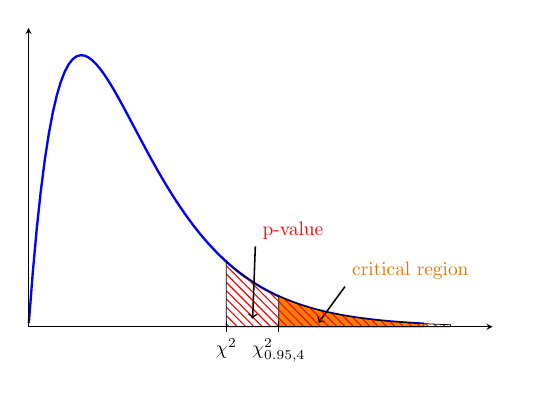
\begin{tikzpicture}[scale=.7,
		declare function={
		  gamma(\z)=2.506628274631*sqrt(1/\z)+ 0.20888568*(1/\z)^(1.5)+ 0.00870357*(1/\z)^(2.5)- (174.2106599*(1/\z)^(3.5))/25920- (715.6423511*(1/\z)^(4.5))/1244160)*exp((-ln(1/\z)-1)*\z;
		},
		declare function={
		 chisq(\x,\k) = exp((0.5*\k-1.0)*ln(\x) - 0.5*\x - gamma(0.5*\k) - \k*0.5*ln(2));
		}
		]
		\begin{axis}[
		  height=7cm, width=10cm,
		  axis x line=center,
		  axis y line=center,
		  xlabel=$$,
		  xtick={7.5, 9.4877},
		  xticklabels={$\chi^2$, $\chi^2_{0.95,4}$},
		  ytick=\empty,
		  x label style={anchor=west},
		  y label style={anchor=south},
		  axis lines=left,
		  axis on top,
		  enlargelimits=upper,
		  samples=100,
		  xmin=0, ymin=0,
		  domain=0.01:15,
		  legend cell align=left,
		  clip=false,
		  major tick length= 2mm,
		  every tick/.style={
			black,thick,}		  
		  ]
		  \addplot [very thick,blue] {chisq(x,4)}; %\addlegendentry{$k=1$}
		  \addplot [ fill=orange,domain=9.4877:15] {chisq(x,4)} \closedcycle ;
		  \draw[<-, thick] (axis cs: 11,.001) -- (axis cs: 12,.01) node [above right] {\og critical region};
		  \addplot [pattern = north west lines, pattern color=red,domain=7.5:16] {chisq(x,4)} \closedcycle ;
		  \draw[<-, thick] (axis cs: 8.5,.002) -- (axis cs: 8.6,.02) node [above right, align=left] {\rd p-value};
		  % \addplot [very thick,purple] {chisq(x,7)}; \addlegendentry{$k=6$}
		\end{axis}
	  \end{tikzpicture}    	
	\end{minipage}
	\begin{minipage}{.4\textwidth}
		Since the test statistic, \pause $\chi^2 = 7.5 \pause < \chi^2_{0.95,4} = 9.4877$, then the test statistic is in the region of non-rejection. \pause

		We can therefore say that the $p$-value $> 0.05$. \pause

		\alert{But how much greater?}
	\end{minipage}

   
  \end{exampleblock}
\end{frame}


\begin{frame}
  \frametitle{Working with the chi-square distribution (cont.)}
  \begin{exampleblock}{Example 3: $p$-value (cont.)}\pause

    We can increase $\alpha$ further and try $\alpha = 0.10$. Thus: \pause

    \begin{equation*}
      \chi^2_{0.90,4} = {\og \mathtt{chi2inv(.9, 4)}} =  7.7794
    \end{equation*}
    \pause
	\begin{minipage}{.5\textwidth}
		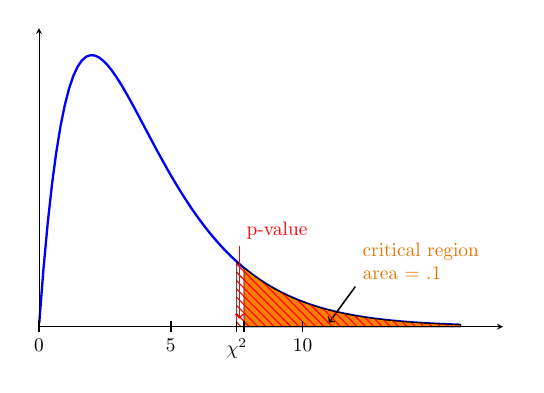
\begin{tikzpicture}[scale=.7,
			declare function={
			  gamma(\z)=2.506628274631*sqrt(1/\z)+ 0.20888568*(1/\z)^(1.5)+ 0.00870357*(1/\z)^(2.5)- (174.2106599*(1/\z)^(3.5))/25920- (715.6423511*(1/\z)^(4.5))/1244160)*exp((-ln(1/\z)-1)*\z;
			},
			declare function={
			 chisq(\x,\k) = exp((0.5*\k-1.0)*ln(\x) - 0.5*\x - gamma(0.5*\k) - \k*0.5*ln(2));
			}
			]
			\begin{axis}[
			  height=7cm, width=10cm,
			  axis x line=center,
			  axis y line=center,
			  xlabel=$$,
			  xtick={0, 5, 7.5, 7.7794, 10},
			  xticklabels={0, 5, $\chi^2$, $$, 10},
			  ytick=\empty,
			  x label style={anchor=west},
			  y label style={anchor=south},
			  axis lines=left,
			  axis on top,
			  enlargelimits=upper,
			  samples=100,
			  xmin=0, ymin=0,
			  domain=0.01:16,
			  legend cell align=left,
			  clip=false,
			  major tick length= 2mm,
			  every tick/.style={
				black,thick,}
			  ]
			  \addplot [very thick,blue] {chisq(x,4)}; %\addlegendentry{$k=1$}
			  \addplot [ fill=orange,domain=7.7794:16] {chisq(x,4)} \closedcycle ;
			  \draw[<-, thick] (axis cs: 11,.001) -- (axis cs: 12,.01) node [above right, align=left] {\og critical region\\ \og
			  area = .1};
			  \addplot [pattern = north west lines, pattern color=red,domain=7.5:16] {chisq(x,4)} \closedcycle ;
			  \draw[<-, red, thick] (axis cs: 7.6,.002) -- (axis cs: 7.6,.02) node [above right, align=left] {\rd p-value};
			  % \addplot [very thick,purple] {chisq(x,7)}; \addlegendentry{$k=6$}
			\end{axis}
		  \end{tikzpicture}    	
		\end{minipage}
		\begin{minipage}{.4\textwidth}
			We see that the critical value is still greater than $\chi^2$, but the difference is much smaller. \pause
			\begin{equation*}
			  \chi^2 = 7.5 \pause < \chi^2_{0.90,4} = 7.7794
			\end{equation*}
			Thus, we can say that the $p$-value is quite close to 0.10.\pause
		\end{minipage}
	



 
  \end{exampleblock}
\end{frame}

\begin{frame}
	\frametitle{Working with the chi-square distribution (cont.)}
	\begin{exampleblock}{Example 3: $p$-value (cont.)}\pause
  
		We can also see that $\chi^2_{.8,4} = {\og \mathtt{chi2inv(.8, 4)}} = 5.9886$. \pause This is evidence that the $p$-value is not greater than 0.20. \pause

		\begin{minipage}{.55\textwidth}
		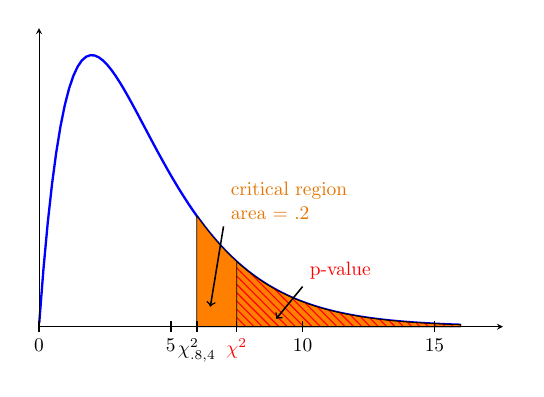
\begin{tikzpicture}[scale=.7,
			declare function={
			  gamma(\z)=2.506628274631*sqrt(1/\z)+ 0.20888568*(1/\z)^(1.5)+ 0.00870357*(1/\z)^(2.5)- (174.2106599*(1/\z)^(3.5))/25920- (715.6423511*(1/\z)^(4.5))/1244160)*exp((-ln(1/\z)-1)*\z;
			},
			declare function={
			 chisq(\x,\k) = exp((0.5*\k-1.0)*ln(\x) - 0.5*\x - gamma(0.5*\k) - \k*0.5*ln(2));
			}
			]
			\begin{axis}[
			  height=7cm, width=10cm,
			  axis x line=center,
			  axis y line=center,
			  xlabel=$$,
			  xtick={0, 5, 5.9886, 7.5,  10, 15},
			  xticklabels={0, 5,  $\chi^2_{.8,4}$, $\rd\chi^2$, 10, 15},
			  ytick=\empty,
			  x label style={anchor=west},
			  y label style={anchor=south},
			  axis lines=left,
			  axis on top,
			  enlargelimits=upper,
			  samples=100,
			  xmin=0, ymin=0,
			  domain=0.01:16,
			  legend cell align=left,
			  clip=false,
			  major tick length= 2mm,
			  every tick/.style={
				black,thick,}
			  ]
			  \addplot [very thick,blue] {chisq(x,4)}; %\addlegendentry{$k=1$}

			  \addplot [ fill=orange,domain=5.9886:16] {chisq(x,4)} \closedcycle ;
			  \draw[<-, thick] (axis cs: 6.5,.005) -- (axis cs: 7,.025) node [above right, align=left] {\og critical region\\ \og
			  area = .2};
			  \addplot [pattern = north west lines, pattern color=red,domain=7.5:16] {chisq(x,4)} \closedcycle ;
			  \draw[<-, thick] (axis cs: 9,.002) -- (axis cs: 10,.01) node [above right, align=left] {\rd p-value};

			  % \addplot [very thick,purple] {chisq(x,7)}; \addlegendentry{$k=6$}
			\end{axis}
		  \end{tikzpicture}
		\end{minipage}		\pause
		  \begin{minipage}{.4\textwidth}
			From MATLAB, we find that the $p$-value is given by \texttt{chi2cdf(7.5,4,'upper')}:\pause
			\begin{equation*}
			  F(\chi^2,k) = F(7.5, 4) = \boxed{0.1117}
			\end{equation*}		
		\end{minipage}
		
		\pause
		\alert{ Note that $F$ here represents the CDF of the $\chi^2$ distribution (not the $F$ distribution).}

	\end{exampleblock}
  \end{frame}

 


\section{Goodness of fit for distributions}
\begin{frame}
  \frametitle{Goodness-of-fit testing}

  \begin{itemize}

  \item Chi-square tests can be used to examine whether data from a sample fit  expected values from a theoretical model/distribution
  \pause

  \item  If the null hypothesis that the observed frequencies are equal to their theoretical counterparts, then the test statistic follows a chi-square distribution, and thus we use it to conduct the hypothesis test
  \pause
  
  %We prescribe that $e_i \ge 5$ for satisfactory results. 
  \item 

  Generally, we can write the {\bf test statistic} as:

  \begin{equation}
    \label{eq:20}
    \chi^2 = \sum_{i=1}^k \fr{(o_i - e_i)^2}{e_i}
  \end{equation}

  \pause

  where $o_i$ is the number of observations in each group or interval $i$,{} \pause and $e_i$ is the expected/theoretical frequency for each group/interval.

  \item The $k$ (degrees of freedom) parameter is given by $k = k-1$.

\end{itemize}
\end{frame}

\begin{frame}
	\frametitle{Test statistic}
	Given $n$ observations with expected probabilities $p_{i0}$, the statistic:\pause
	\begin{equation}
	  \label{eq:1}
	  \chi^2 = \sum \fr{(\text{observed} - \text{expected})^2}{\text{expected}} \pause = \sum_{i=1}^k \fr{(o_i - np_{i0})^2}{np_{i0}}
	\end{equation}
	is approximately \textbf{chi-square} distributed with $k = k-1$, {\bf provided that $np_i \ge 5$ for all $i$}.
  \end{frame}


\begin{frame}
  \frametitle{Steps to perform chi-square goodness-of-fit tests}\pause
  \begin{enumerate}[\bf Step 1.]
  \item Order/sort the observations (if necessary) \pause
  \item Group the observations (or aggregate into reasonable intervals) \pause
  \item Find the frequencies for each group \pause
  \item Compute the theoretical frequencies for each group: 
  \begin{equation}
	n \times P(a_i < X \le b_i)
  \end{equation}
 	  \pause
  \item Compute the chi-square statistic: 
 \begin{equation}
	\chi^2 = \sum_{i=1}^k \fr{(o_i - e_i)^2}{e_i}
 \end{equation} 
   \pause
  \item Perform the hypothesis test and conclude
  \end{enumerate}
\end{frame}



\begin{frame}
  \frametitle{Goodness-of-fit testing}
  \begin{exampleblock}{Example 4: Peas in a pod}
      The distribution of the dominant alleles (forms of a gene) in peas (Y = yellow color, R = round shape) is binomial with $p = \fr{9}{16}$.
      An experiment was performed to test the hypothesis that all the observed frequencies are equal to the theoretical ones (null hypothesis) versus the alternative that at least one is not.
      In this experiment, $n$ four-seed pods were examined. In a randomly selected pod, possible $X$ values were 0, 1, 2, 3 and 4.

      The following data are given ({\bf one-way table}):\\

      \begin{minipage}{.6\textwidth}
              {\centering
        \begin{tabular}{| l | c | c | c | c | c|}\hline
          \bf Cell $\bm i$ & \bf 1 & \bf 2 & \bf 3 & \bf 4 & \bf 5 \\ \hline
          \bf YR peas/pods & \bf 0 & \bf 1 & \bf 2 & \bf 3 & \bf 4 \\ \hline
          Observed         & 16    & 45    & 100   &  82   &  26   \\ \hline
          Expected         &       &       &       &       &       \\ \hline
          $(o_i - e_i)^2/e_i$ &     &      &  & & \\ \hline
        \end{tabular}
      }
      \end{minipage}
      \begin{minipage}{.35\textwidth}
        \includegraphics[width=\textwidth]{peas.png}

        {\tiny Source: \href{https://www.biologycorner.com/bio2/genetics/notes_mendel.html}{Biology Corner}}
      \end{minipage}
    
      \bigskip
      Complete the table and perform the hypothesis test at level 0.01 ($\alpha$).
  \end{exampleblock}
\end{frame}

\begin{frame}
  \frametitle{Goodness-of-fit testing}
  \begin{exampleblock}{Example 4: Peas in a pod (cont.)}\pause
    Given $n= 16  + 45  + 100  +   82 + 26 =269$, we compute the theoretical frequencies:\pause
    \begin{eqnarray*}
      e_i &=&  n\times {n \choose i-1} p^{i-1}(1 - p)^{4 - (i-1)} \\ \pause
      e_1 &=& 269 \times {4\choose 0}\lt(\fr9{16}\rt)^0\lt(\fr7{16}\rt)^{4} = \pause 9.86 \\\pause
      e_2 &=& 269 \times {4\choose 1}\lt(\fr9{16}\rt)^1\lt(\fr7{16}\rt)^{3} = \pause 50.38 \\\pause
      e_3 &=& 269 \times {4\choose 2}\lt(\fr9{16}\rt)^2\lt(\fr7{16}\rt)^{2} = \pause 97.75 \\\pause
      e_4 &=& 269 \times {4\choose 3}\lt(\fr9{16}\rt)^3\lt(\fr7{16}\rt)^{1} = \pause 83.78 \\\pause
      e_5 &=& 269 \times {4\choose 4}\lt(\fr9{16}\rt)^4\lt(\fr7{16}\rt)^{0} = \pause 26.93
    \end{eqnarray*}
  \end{exampleblock}
\end{frame}


\begin{frame}
  \frametitle{Goodness-of-fit testing}
  \begin{exampleblock}{Example 4: Peas in a pod (cont.)}\pause

    Our updated table is now: \pause

    
      {\centering
        \begin{tabular}{| l | c | c | c | c | c|}\hline
          \bf Cell $\bm i$ & \bf 1 & \bf 2 & \bf 3 & \bf 4 & \bf 5 \\
          \bf YR peas/pods & \bf 0 & \bf 1 & \bf 2 & \bf 3 & \bf 4 \\ \hline
          Observed         & 16    & 45    & 100   &  82   &  26   \\ \hline
          Expected         & 9.86  & 50.38 & 97.75 & 83.78 &  26.93  \\ \hline
          $(o_i - e_i)^2/e_i$ &     &      &  & & \\ \hline
        \end{tabular}
      }
      \pause

      \bigskip
      
      We can then compute the normalized squared deviations\pause
  \end{exampleblock}
\end{frame}




\begin{frame}
  \frametitle{Goodness-of-fit testing}
  \begin{exampleblock}{Example 4: Peas in a pod (cont.)}\pause
    \begin{eqnarray*}
      (n_1 - e_1)^2/e_1 &=& \pause (16 - 9.86)^2/9.86 \pause = 3.823 \\ \pause
      (n_2 - e_2)^2/e_2 &=& \pause (45 - 50.68)^2/50.68 \pause = 0.637 \\ \pause
      (n_3 - e_3)^2/e_3 &=& \pause (100 - 97.75)^2/97.75 \pause = 0.052 \\ \pause
      (n_4 - e_4)^2/e_4 &=& \pause (82 - 83.78)^2/83.78 \pause = 0.038 \\ \pause
      (n_5 - e_5)^2/e_5 &=& \pause (26 - 26.93)^2/26.93 \pause = 0.032
    \end{eqnarray*}
  \end{exampleblock}
\end{frame}


\begin{frame}
  \frametitle{Goodness-of-fit testing}
  \begin{exampleblock}{Example 4: Peas in a pod (cont.)}\pause
    Now, we have all we need to compute the chi-square test statistic: \pause
    \begin{eqnarray*}
      \chi^2 &=& \sum_{i=1}^G (o_i - e_i)^2/e_i \\ \pause
             &=& 3.823 + 0.637 + 0.052 + 0.038 + 0.032 \\  \pause
             &=& 4.582
    \end{eqnarray*}
    \pause
	The degrees of freedom, $k = G- 1 = 5-1 = 4$. \pause 

    Thus, the critical value is given by $\chi^2_{0.99, 4} = \pause 13.2767$.
  \end{exampleblock}
\end{frame}


\begin{frame}
  \frametitle{Goodness-of-fit testing}
  \begin{exampleblock}{Example 4: Peas in a pod (cont.)}
    Since $\chi^2 = 4.582 \pause < \chi^2_{0.99, 4} = \pause 13.2767$, we \textbf{fail to reject} the null hypothesis. \pause

    This indicates that the binomial model is a good fit for the data. \pause

          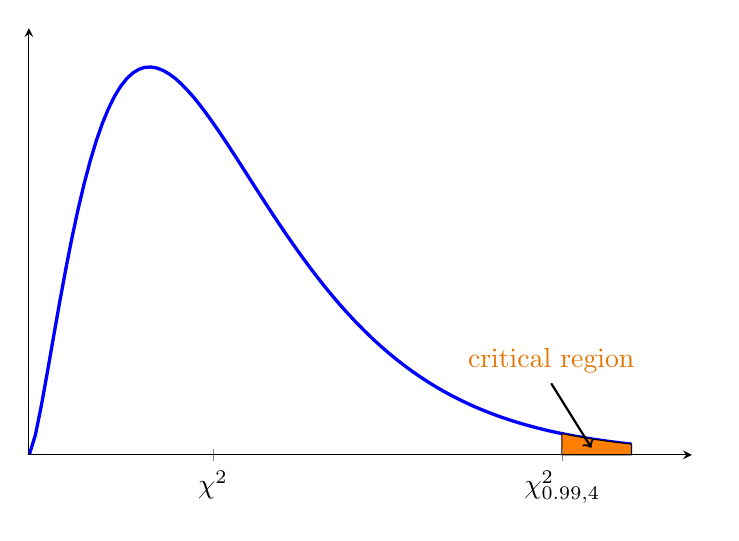
\begin{tikzpicture}[scale=1,
      declare function={
        gamma(\z)=2.506628274631*sqrt(1/\z)+ 0.20888568*(1/\z)^(1.5)+ 0.00870357*(1/\z)^(2.5)- (174.2106599*(1/\z)^(3.5))/25920- (715.6423511*(1/\z)^(4.5))/1244160)*exp((-ln(1/\z)-1)*\z;
      },
      declare function={
       chisq(\x,\k) = exp((0.5*\k-1.0)*ln(\x) - 0.5*\x - gamma(0.5*\k) - \k*0.5*ln(2));
      }
      ]
      \begin{axis}[
        height=7cm, width=10cm,
        axis x line=center,
        axis y line=center,
        xlabel=$$,
        xtick={4.582, 13.2767},
        xticklabels={$\chi^2$, $\chi^2_{0.99,4}$},
        ytick=\empty,
        x label style={anchor=west},
        y label style={anchor=south},
        axis lines=left,
        axis on top,
        enlargelimits=upper,
        samples=100,
        xmin=0, ymin=0,
        domain=0.01:15,
        legend cell align=left,
        clip=false
        ]
        \addplot [very thick,blue] {chisq(x,5)}; %\addlegendentry{$k=1$}
        \addplot [ fill=orange,domain=13.267:15] {chisq(x,5)} \closedcycle ;
        \draw[<-, thick] (axis cs: 14,.001) -- (axis cs: 13,.01) node [above] {\og critical region};
        % \addplot [very thick,purple] {chisq(x,7)}; \addlegendentry{$k=6$}
      \end{axis}
    \end{tikzpicture}    
  \end{exampleblock}
\end{frame}

\begin{frame}
  \frametitle{Example 5}
  \pause
  We will revisit Scenario 2 as an in-class activity:

  \begin{itemize}
    \item Each of you will be assigned to a group
    \item In your group, count the following:
    \begin{itemize}
      \item number of CEE majors ($\hat{n}_A$)
      \item number of ME majors ($\hat{n}_B$)
      \item number of IE majors ($\hat{n}_C$)
      \item number of Other majors ($\hat{n}_D$)
    \end{itemize}
    \item Goal: test whether the distribution of majors in your sample (group) is representative of the expected (true) counts ($n_A, n_B, n_C, n_D$) based on the proportions obtained from the class-wide survey you just completed.
  \end{itemize}

  

\end{frame}
\section{Outlook}
\begin{frame}
\frametitle{Summary}
\begin{itemize}
	\item The $\chi^2$ distribution has a single parameter $k$ (degrees of freedom)
	\item It is the underlying the distribution for chi-square tests, which are used to evaluate whether observed data fit a given distribution (or that proportions/frequencies observed from a sample follow a theoretical model/assumption).
	\item Critical value: $\chi^2_{1-\alpha, k} \equiv \pythoninline{chi2.ppf(1-alpha, k)}$
	\item p-value: \pythoninline{chi2.cdf(test, k)}
	\item When given a one-way table, the test statistic $\chi^2$ is computed as
 \begin{equation}
	\chi^2 = \sum_{i=1}^G \fr{(o_i - e_i)^2}{e_i}, \quad k = G - 1
 \end{equation} 
 where $G$ is the number of groups
 \item Reject null hypothesis: p-value $< \alpha $ OR $ \chi^2 > \chi^2_{1-\alpha, k} $
 \item Fail to reject null hypothesis: p-value $\geq \alpha $ OR $\chi^2 \leq \chi^2_{1-\alpha, k}  $
 \item Reading: Open Intro Stats, Section 6.3
\end{itemize}
\end{frame}

\end{document}
%%% Local Variables:
%%% mode: latex
%%% TeX-master: t
%%% End:
